\documentclass[12pt,a4paper]{article}
\usepackage{graphicx}
\usepackage{amsmath}
\usepackage{amssymb}
\usepackage{algorithm}
\usepackage{algorithmic}
\usepackage{float}
\usepackage{cite}
\usepackage{url}
\usepackage{booktabs}
\usepackage{array}
\usepackage{multirow}
\usepackage{geometry}
\usepackage{hyperref}
\usepackage{caption}
\usepackage{subcaption}
\usepackage{xcolor}
\usepackage{tikz}
\usepackage{pgfplots}
\pgfplotsset{compat=1.18}

\geometry{margin=1in}

\hypersetup{
	colorlinks=true,
	linkcolor=blue,
	citecolor=blue,
	urlcolor=blue
}

\title{\textbf{An EM-Based Multi-Task Ensemble Framework for Adaptive Concept Drift Detection in Data Streams}}

\author{H. Sadoghi Yazdi, Department of Computer Engineering, Faculty of Engineering, Center of Excellence in Soft Computing and Intelligent Information Processing, Ferdowsi University of Mashhad, Mashhad, Iran (e-mail: h-sadoghi@um.ac.ir}



\begin{document}
	
	\maketitle
	
	\begin{abstract}
		The rapid growth of streaming data in dynamic environments necessitates classifiers that can efficiently handle concept drift while maintaining high predictive performance under strict resource constraints. Traditional single-model or fixed-ensemble approaches often fail to adapt quickly to various types of drift (abrupt, gradual, recurring, or incremental).
		
		In this paper, we propose \textbf{EM-MTE}, an \textbf{Expectation-Maximization based Multi-Task Ensemble} framework for concept-drifting data streams. We model the streaming problem as a multi-task learning scenario where each drift-sensitive objective or data block/view is treated as a task. A shared library of online learning components (e.g., Perceptron, Passive-Aggressive, Confidence-Weighted models) is dynamically combined for each task through latent responsibility variables. These responsibilities are iteratively estimated via the EM algorithm, enabling principled, adaptive, and task-specific weighting of experts.
		
		The proposed method provides a probabilistic interpretation of component combination, closed-form updates in the M-step, and natural handling of uncertainty in non-stationary environments. Extensive experiments on benchmark datasets from the UCI repository and real-world malicious web page detection demonstrate that EM-MTE achieves superior adaptation speed and accuracy compared to state-of-the-art streaming ensembles, while maintaining low memory and computational overhead.
		
		Our framework bridges the gap between theoretical multi-task mixture modeling and practical online concept drift adaptation, offering robustness to label scarcity and different drift patterns.

		
		\medskip
		\noindent\textbf{Keywords:} Concept drift; Data stream; Online learning; Multi-task learning; Ensemble method; Expectation-Maximization
	\end{abstract}
	
	% ---------------------------------------------------------------
	\section{Introduction}
	% ---------------------------------------------------------------
	
	Optimal models for the data mining approach remain a challenging problem for computational intelligence researchers. Traditional methods for processing continuous data have several limitations: (i) data must be stored, (ii) processing is done on stored data based on appropriate parameters. In the static approach, the entire dataset is required which, as time passes, causes computational challenges such as large memory usage, limited processing time, high dimensionality, and continuous change of infinite data~\cite{Krawczyk2017}. Specific examples of data mining in the real world include image processing of satellite pictures, GPS systems, data security events such as spam detection systems, and information retrieval from text, etc.
	
	Adapting to the behavior of arriving data is the most important feature of data stream approaches. These approaches track variations of the loaded data over time. In the process of data flow, a proper model must be trained on the current data to extract new unseen patterns. In online approaches, the feature weights of incoming data are updated to values suitable for prediction. Concept drift refers to a non-stationary and dynamic environment in which the distribution of data often changes over time~\cite{Escovedo2018}. In concept drift, there is no change in the marginal data distribution, but there is a difference in the conditional distribution of the target given the arriving input. A real-world example of concept drift occurs when the attention of users on a social network to some topic is changing. The conditional distribution of users' attention without change in the overall distribution is continuously shifting. There are many adaptive learning approaches aimed at reacting to concept drift; single and ensemble approaches are two main types~\cite{Farid2013}.
	
	In the single-base method, one model is used for the sequence of arriving data, whereas the ensemble method combines basic models simultaneously. Decision trees, sliding windows of sample-based learning, Naive Bayes, and neural networks are examples of the single-base method; AdaBoost, Random Forest, and cluster combiner methods are examples of ensemble-based methods. In single-base rather than ensemble-based approaches, complex models are often used to recognize the pattern of the data stream~\cite{Babcock2002}. Several efficient classifiers can be applied to make ensemble models tractable for the streaming problem.
	
	The importance of concept drift originates in the speed of adaptation needed to create a model. In this paper, because of the changing behavior of data over time and insufficient storage resources for the volume of data, online learning-based algorithms are used. Our system uses real-time modeling following the concept track. Our system can adapt to new behavior given the input data. Our principal research contributions are summarized as follows:
	
	\begin{itemize}
		\item Our system can adapt to the change in input data without the need for additional resources.
		\item Our system is capable of producing suitable real-time modeling when the volume of incoming data arrives quickly.
		\item To present an adaptive system, we propose an aggregation method based on the ensemble prediction of online experts.
		\item When we do not have an accurate label, our system tends to be robust against it.
		\item Our system was tested on benchmark and real datasets and compared to other existing models.
	\end{itemize}
	
	The rest of the paper is organized as follows: Section~\ref{sec:related} reviews existing related work on concept drift. Section~\ref{sec:proposed} demonstrates the proposed EM-based multi-task ensemble for data streams. Section~\ref{sec:evaluation} describes the implementation and experimental results. Finally, Section~\ref{sec:conclusion} presents the conclusion.
	
	% ---------------------------------------------------------------
	\section{Related Work}
	\label{sec:related}
	% ---------------------------------------------------------------
	
	In the real world, different types of concept drift occur. For example, in intrusion detection systems, attackers continuously change their strategies~\cite{Liang2017}. The core categories of algorithms for concept drift distribution can be stated as follows:
	\begin{enumerate}
		\item \textbf{Immediate drift}: recognizing a quick change of the current stream.
		\item \textbf{Gradual drift}: unclear what kind of techniques are required for a re-duplicative bag of input data when there is a slow change in data distribution.
		\item \textbf{Replicating drift}: when some patterns in the data stream repeat permanently.
		\item \textbf{Development drift}: the incoming data stream pattern incrementally changes to another one.
	\end{enumerate}
	
	\begin{figure}[H]
		\centering
		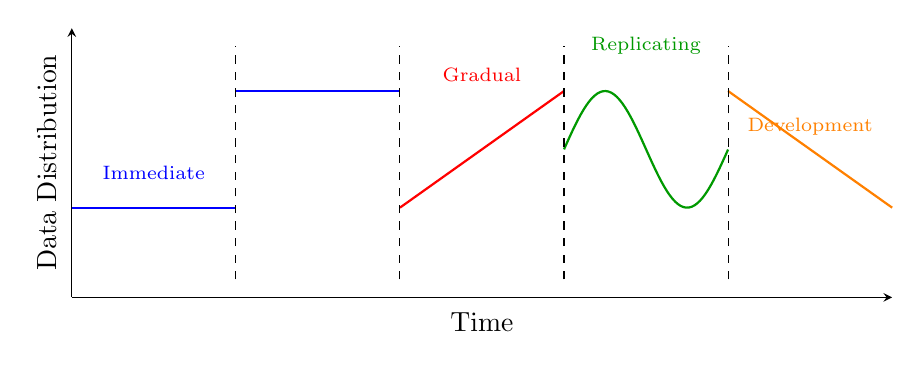
\begin{tikzpicture}
			\begin{axis}[
				width=12cm, height=5cm,
				xlabel={Time},
				ylabel={Data Distribution},
				xtick=\empty,
				ytick=\empty,
				xmin=0, xmax=10,
				ymin=-0.5, ymax=2.5,
				axis lines=left,
				clip=false
				]
				% Immediate drift
				\addplot[thick, blue, domain=0:2] {0.5};
				\addplot[thick, blue, domain=2:4] {1.8};
				\node[above, blue] at (axis cs:1,0.7) {\scriptsize Immediate};
				
				% Gradual drift
				\addplot[thick, red, domain=4:6, samples=50] {0.5 + 1.3*(x-4)/2};
				\node[above, red] at (axis cs:5,1.8) {\scriptsize Gradual};
				
				% Replicating drift
				\addplot[thick, green!60!black, domain=6:8, samples=60] {1.15 + 0.65*sin(deg(3.14*(x-6)))};
				\node[above, green!60!black] at (axis cs:7,2.1) {\scriptsize Replicating};
				
				% Development drift
				\addplot[thick, orange, domain=8:10, samples=50] {1.8 - 1.3*(x-8)/2};
				\node[above, orange] at (axis cs:9,1.2) {\scriptsize Development};
				
				\draw[dashed] (axis cs:2,-0.3) -- (axis cs:2,2.3);
				\draw[dashed] (axis cs:4,-0.3) -- (axis cs:4,2.3);
				\draw[dashed] (axis cs:6,-0.3) -- (axis cs:6,2.3);
				\draw[dashed] (axis cs:8,-0.3) -- (axis cs:8,2.3);
			\end{axis}
		\end{tikzpicture}
		\caption{The types of concept drift in an incoming data stream.}
		\label{fig:concept_drift}
	\end{figure}
	
	Most of the works in stream processing contain sliding windows to display the concept drift~\cite{Sun2017,Torquati2017}. With sliding windows, we take an arriving data query group as the input to the model and then learn the optimal parameters for its concept drift~\cite{Ross2012}. Domingos et al. proposed a Very Fast Decision Tree (VFDT) for detecting sliding window changes in compound data for quick action recognition without the need for using large numbers of out-of-date data~\cite{Domingos2000}. Hulten et al. proposed a system based on the CVFDT algorithm to cope with concept drift; they used a decision tree to model the streaming data, and whenever data change occurs, the newest subtree replaces the previous subtree and updates the node~\cite{Hulten2001}. For determining the number of data by sliding windows, they used the Hoeffding bound; in other approaches, a fixed size is used to examine the newest nodes of the tree. The Hoeffding Adaptive Tree (HAT) and the Hoeffding Window Tree (HWT) are alternative versions of Hoeffding bounds for incrementally changing the number of sliding windows, proposed by Bifet~\cite{Bifet2009}. Mena-Torres et al. proposed a similarity-based method called SimC to classify the input data~\cite{Mena2014}. In their system, an instance-based technique is applied in situations of implicit concept drift. SimC's calculations are based on principles that: (i) each class of data must be grouped together by its attribute, (ii) the distance between each group is calculated, and (iii) older groups are eliminated by calculating age, which influences accuracy.
	
	Other methods, such as cluster methods, have been used for adaptation. Tennant et al. proposed a new technique called Micro-Cluster Nearest Neighbor (MCNN) for classifying data streams. The structure of their system is based on the Nearest Neighbor (NN), which creates micro-clusters to continue adoption~\cite{Tennant2017}. Each micro-cluster depends on the label of the cluster, an error threshold, and the performance of each micro-cluster.
	
	Gama et al. introduced a method called DDM for combining online algorithms such as the perceptron, a neural network, and a decision tree; the feedback of each online learning algorithm is applied to the combination procedure~\cite{Gama2004}. Baena-Garc\'{i}a et al. proposed a new approach (EDDM) similar to DDM, with two differentiating factors: (i) they employ both online learning and batch algorithms, and (ii) similar to DDM, the combination is based on the distance of each classification error~\cite{Baena2006}. Ross et al. chose the classification error rate for detecting concept drift, using the Exponentially Weighted Moving Average (EWMA)~\cite{Ross2012}. In their system, an online classifier is applied to the investigation of data features for a generalized solution to the concept drift problem. EWMA represents concept drift based on a sequence of Bernoulli random variables.
	
	
	
	
	
	% ---------------------------------------------------------------
	\section{The Proposed System}
	\label{sec:proposed}
	% ---------------------------------------------------------------
	
	A significant issue in concept drift detection is the reliability of functional algorithms with minimum delay and storage usage. In this paper, the proposed method is reformulated as an \textit{EM-based multi-task ensemble}. The central idea is that a data stream is not handled by one global online model or by a fixed averaging of experts. Instead, each drift-sensitive prediction objective is treated as a task, and each task learns a soft combination of shared online components. The combination weights are estimated by the Expectation-Maximization (EM) principle through latent responsibility variables.
	
	We assume that the incremental input stream constructs the dataset $D$ where:
	\[
	D = \{(I_t;\, L_t) \mid I_t \in \mathbb{R}^d,\; L_t \in \{-1, +1\},\; t = 1, 2, \ldots, n\}
	\]
	and $I_t$ is each incoming instance at time $t$ and $L_t$ is its label. The stream is divided into sequential blocks $S=\{s_1,\ldots,s_B\}$. Each block, drift type, label view, or application objective can define a task. We denote the set of tasks by $\mathcal{T}=\{1,\ldots,T\}$ and the dataset assigned to task $r$ by
	\[
	\mathcal{D}^{(r)}=\{(x_i^{(r)},y_i^{(r)})\}_{i=1}^{N_r}.
	\]
	In the streaming case, $x_i^{(r)}$ is obtained from $I_t$, and $y_i^{(r)}$ is the corresponding label or task-specific target. The method uses $K$ shared components $\{C_1,\ldots,C_K\}$. A component can be a linear-order learner, such as Perceptron, OGD, and Passive-Aggressive models, or a Gaussian-order learner, such as CW, AROW, SOP, and related confidence-weighted models. These components form an ensemble library, but the ensemble is not fixed: every task has its own mixture weights over the same library.
	
	\begin{figure}[H]
		\centering
		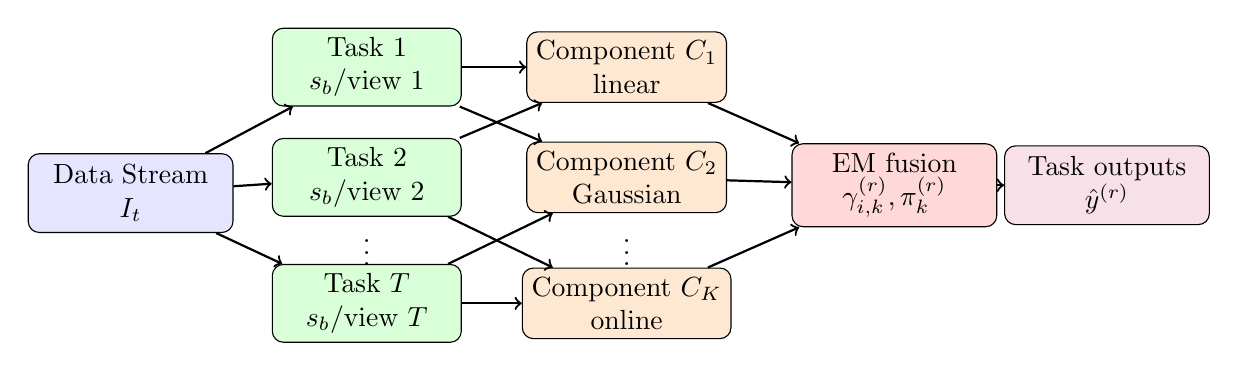
\begin{tikzpicture}[
			box/.style={draw, rounded corners, minimum width=2.6cm, minimum height=1cm, align=center, fill=blue!10},
			task/.style={draw, rounded corners, minimum width=2.4cm, minimum height=0.8cm, align=center, fill=green!15},
			comp/.style={draw, rounded corners, minimum width=2.1cm, minimum height=0.8cm, align=center, fill=orange!18},
			arrow/.style={->, thick}
			]
			\node[box] (input) at (0,0) {Data Stream\\$I_t$};
			\node[task] (t1) at (3,1.6) {Task 1\\$s_b$/view 1};
			\node[task] (t2) at (3,0.2) {Task 2\\$s_b$/view 2};
			\node[task] (tT) at (3,-1.4) {Task $T$\\$s_b$/view $T$};
			\node at (3,-0.65) {$\vdots$};
			\node[comp] (c1) at (6.3,1.6) {Component $C_1$\\linear};
			\node[comp] (c2) at (6.3,0.2) {Component $C_2$\\Gaussian};
			\node[comp] (cK) at (6.3,-1.4) {Component $C_K$\\online};
			\node at (6.3,-0.65) {$\vdots$};
			\node[box, fill=red!15] (em) at (9.7,0.1) {EM fusion\\$\gamma_{i,k}^{(r)},\pi_k^{(r)}$};
			\node[box, fill=purple!12] (out) at (12.4,0.1) {Task outputs\\$\hat{y}^{(r)}$};
			\draw[arrow] (input) -- (t1);
			\draw[arrow] (input) -- (t2);
			\draw[arrow] (input) -- (tT);
			\draw[arrow] (t1) -- (c1);
			\draw[arrow] (t1) -- (c2);
			\draw[arrow] (t2) -- (c1);
			\draw[arrow] (t2) -- (cK);
			\draw[arrow] (tT) -- (c2);
			\draw[arrow] (tT) -- (cK);
			\draw[arrow] (c1) -- (em);
			\draw[arrow] (c2) -- (em);
			\draw[arrow] (cK) -- (em);
			\draw[arrow] (em) -- (out);
		\end{tikzpicture}
		\caption{Overall view of the proposed EM-based multi-task ensemble. Tasks are routed to a shared component library, and EM estimates task-specific responsibilities and mixture weights.}
		\label{fig:em_mtl_stream_overview}
	\end{figure}
	
	\subsection{Online Components as Shared Task Solvers}
	
	Perceptron is an online algorithm based on the feedback of one hidden layer for streaming data~\cite{Irie1988}. Another similar approach is OGD (Online Gradient Descent), which is based on minimizing the gradient of incoming data~\cite{Zinkevich2003}. The weaknesses of Perceptron and OGD are in identifying incremental and sudden drift, respectively. The use of different types of Passive-Aggressive (PA) algorithms can be considered to improve concept drift detection~\cite{Crammer2006}. In the proposed model, these online learners are not independent final classifiers; they are shared components that can be reused by several tasks with different responsibilities. For a PA component, the best weight parameter in every iteration is obtained by solving
	\begin{equation}
		w_{t+1} = \arg\min_{W \in \mathbb{R}^d}\; \frac{1}{2}\|W - w_t\|^2 \quad \text{s.t.}\quad L_t\,(w_t \cdot I_t) \geq 1
		\label{eq:pa_opt}
	\end{equation}
	
	The loss function and input value are important driving factors for determining the model. In each round, the model trends towards the best weight incrementally. By solving the optimization problem in Eq.~(\ref{eq:pa_opt}), PA updates its model as follows:
	\begin{equation}
		w_{t+1} = w_t + \frac{l_t}{\|I_t\|^2}\,\gamma\, L_t\, I_t
		\label{eq:pa_update}
	\end{equation}
	where $w_{t+1}$ is the new weight based on input data stream; $l_t = \max(0, 1 - L_t\,w_t \cdot I_t)$ is the hinge loss; and $\gamma$ is a parameter which determines the importance of the loss function. Various states of concept drift can be considered using the cost function and other parameters. Types of \textit{linear-order} online learners for concept drift are shown in Table~\ref{tab:linear_order}.
	
	\begin{table}[H]
		\centering
		\caption{Types of \textit{Linear-order} online learning algorithms and their most impactful aspect for concept drift}
		\label{tab:linear_order}
		\renewcommand{\arraystretch}{1.6}
		\resizebox{\textwidth}{!}{%
			\begin{tabular}{|l|l|l|l|}
				\hline
				\textbf{Algorithm} & \textbf{Loss function} & \textbf{Weight update} & \textbf{Concept drift} \\
				\hline
				Perceptron~\cite{Irie1988}
				& $l_t = \max(0, 1 - L_t w_t I_t)$
				& $w_{t+1} = w_t + l_t L_t I_t$
				& Immediate \\
				\hline
				OGD (logistic)~\cite{Zinkevich2003}
				& $l_t = \log(1 + e^{-L_t w_t I_t})$
				& $w_{t+1} = w_t + \gamma\, l_t\, L_t\, I_t$
				& Replicating \\
				\hline
				PA~\cite{Crammer2006}
				& $l_t = \max(0, 1 - L_t w_t I_t)$
				& $w_{t+1} = w_t + \frac{l_t}{\|I_t\|^2}\,\gamma\, L_t I_t$
				& Gradual \\
				\hline
				PA-I~\cite{Crammer2006}
				& $l_t = \max(0, 1 - L_t w_t I_t)$
				& $\gamma_t = \min\!\left(C,\, \frac{l_t}{\|I_t\|^2}\right);\quad w_{t+1} = w_t + \gamma_t L_t I_t$
				& Gradual, Replicating \\
				\hline
				PA-II~\cite{Crammer2006}
				& $l_t = \max(0, 1 - L_t w_t I_t)$
				& $\gamma_t = \frac{l_t}{\|I_t\|^2 + \frac{1}{2C}};\quad w_{t+1} = w_t + \gamma_t L_t I_t$
				& Gradual, Replicating \\
				\hline
				ROMMA~\cite{Li2000}
				& $l_t = \max(0, 1 - L_t w_t I_t)$
				& $\alpha_t = \frac{(\|I_t\|\cdot\|w\|)^2 - L_t(w\cdot I_t)}{(\|I_t\|\cdot\|w\|)^2 - (w\cdot I_t)^2}$;\; $\beta_t = \frac{\|w\|^2\cdot L_t(w\cdot I_t)}{(\|I_t\|\cdot\|w\|)^2 - (w\cdot I_t)^2}$;\; $w_{t+1} = \alpha_t w_t + \beta_t I_t$
				& Immediate, Replicating \\
				\hline
				aROMMA~\cite{Li2000}
				& $l_t = 1 - L_t w_t I_t$
				& (same as ROMMA)
				& Immediate, Replicating \\
				\hline
				ALMA~\cite{Gentile2001}
				& $l_t = (1-\alpha)\frac{1}{\alpha}\sqrt[p-1]{p}\frac{1}{\sqrt{k+1}} - L_t w_t I_t$
				& $\beta_t = \frac{C}{\sqrt[p-1]{p}\sqrt{t}}$;\; $w_{t+1} = w_t + \beta_t L_t I_t$;\; $w_{t+1} \leftarrow \frac{w_{t+1}}{\max(1,\|w_{t+1}\|)}$
				& Replicating \\
				\hline
			\end{tabular}%
		}
	\end{table}
	
	The \textit{Gaussian-order} is the other type of online learning algorithm, which updates parameters based on a Gaussian distribution. The mean vector $\mu \in \mathbb{R}^d$ and covariance matrix $\Sigma \in \mathbb{R}^{d\times d}$ of the input data distribution are the principal factors in determining concept drift. Confidence Weighting (CW) is one of the most popular algorithms for the Gaussian-order~\cite{Dredze2008}. For data streams where we have low variance of the obtained data, CW determines more confidence in the average data. To recognize concept drift in a data stream, the Kullback-Leibler (KL) divergence is used as follows:
	\begin{equation}
		(\mu_{t+1}, \Sigma_{t+1}) = \arg\min_{(\mu,\Sigma)}\; D_{\mathrm{KL}}\bigl(\mathcal{N}(\mu, \Sigma) \;\|\; \mathcal{N}(\mu_t, \Sigma_t)\bigr)
		\quad \text{s.t.} \quad L_t\,(\mu^{\top} I_t) \geq 1
		\label{eq:cw_opt}
	\end{equation}
	
	After solving the cost function in Eq.~(\ref{eq:cw_opt}), the new weighting of each input data is calculated as follows:
	\begin{align}
		w_{t+1} &= w_t + \alpha_t\, L_t\, I_t \cdot \Sigma_t \label{eq:cw_w} \\
		\Sigma_{t+1} &= \Sigma_t - \beta_t\, I_t\, \Sigma_t^{\top} \label{eq:cw_sigma}
	\end{align}
	In these algorithms, the significant parameters $\alpha_t$ and $\beta_t$ depend on the weight and Gaussian distribution of input features, respectively. These are more efficient for computing the loss function. Other types of Gaussian-order online experts are shown in Table~\ref{tab:gaussian_order}.
	
	\begin{table}[H]
		\centering
		\caption{Types of \textit{Gaussian-order} online learning algorithms}
		\label{tab:gaussian_order}
		\renewcommand{\arraystretch}{1.8}
		\resizebox{\textwidth}{!}{%
			\begin{tabular}{|l|l|l|l|}
				\hline
				\textbf{Algorithm} & \textbf{Loss function} & \textbf{Weight update} & \textbf{Concept drift} \\
				\hline
				CW~\cite{Dredze2008}
				& $l_t = \max(0, 1 - L_t w_t I_t)$
				& $\alpha_t = \frac{-\phi l_t + \sqrt{\phi^2 l_t^2 + 4 v_t}}{2 v_t}$;\; $w_{t+1} = w_t + \alpha_t L_t I_t \Sigma_t$;\; $\Sigma_{t+1} = \Sigma_t - \beta_t(\Sigma_t I_t)^2$
				& Gradual, Replicating, Development \\
				\hline
				SCW-I~\cite{Wang2012}
				& $l_t = \phi\sqrt{v_t} - L_t w_t I_t$
				& $\alpha_t = \max\!\left(0,\, \frac{-(\phi^2 l_t v_t + \phi v_t \sqrt{\phi^2 l_t^2 + 4 v_t})}{2(\phi^2 v_t^2 - l_t^2)}\right)$;\; $\alpha_{t+1} = \min(\alpha_t, C)$;\; $w_{t+1} = w_t + \alpha_{t+1} L_t I_t \Sigma_t$;\; $\Sigma_{t+1} = \Sigma_t - \beta_t(\Sigma_t I_t)^2$
				& Gradual, Replicating, Development \\
				\hline
				SCW-II~\cite{Wang2012}
				& $l_t = \phi\sqrt{v_t} - L_t w_t I_t$
				& $\lambda = \sqrt{(\phi^2 v_t^2 + l_t^2)\cdot C}$;\; $\alpha_t = \max(0, \frac{-\phi^2 v_t l_t + \lambda}{\phi^2 v_t + \frac{1}{2C}})$;\; $\alpha_{t+1} = \min(\alpha_t, C)$;\; $w_{t+1}$, $\Sigma_{t+1}$ same as SCW-I
				& Gradual, Replicating, Development \\
				\hline
				AROW~\cite{Crammer2009}
				& $l_t = \max(0, 1 - L_t w_t I_t)$
				& $\alpha_t = \frac{l_t}{I_t^{\top}\Sigma_t I_t + \gamma}$;\; $w_{t+1} = w_t + \alpha_t L_t \Sigma_t I_t$;\; $\Sigma_{t+1} = \Sigma_t - \frac{\Sigma_t I_t I_t^{\top}\Sigma_t}{I_t^{\top}\Sigma_t I_t + \gamma}$
				& Gradual, Replicating, Development \\
				\hline
				NAROW~\cite{Crammer2009}
				& $l_t = 1 - L_t w_t I_t$
				& $\beta_t = \frac{1}{I_t^{\top}\Sigma_t I_t + \frac{1}{\gamma}}$;\; $\alpha_t = \max(0, l_t)\,\beta_t$;\; $w_{t+1} = w_t + \alpha_t L_t \Sigma_t I_t$;\; $\Sigma_{t+1} = \Sigma_t - \beta_t \Sigma_t I_t I_t^{\top}\Sigma_t$
				& Gradual, Replicating, Development \\
				\hline
				SOP~\cite{CesaBianchi2005}
				& $l_t = \max(0, 1 - L_t w_t I_t)$
				& $\beta_t = \frac{1}{I_t^{\top}\Sigma_t I_t + 1}$;\; $\alpha_t = \max(0, l_t)\,\beta_t$;\; $w_{t+1} = w_t + \alpha_t L_t I_t$;\; $\Sigma_{t+1} = \Sigma_t - \beta_t(\Sigma_t I_t)^2$
				& Gradual, Replicating, Development \\
				\hline
				NHERD~\cite{Crammer2010}
				& $l_t = 1 - L_t w_t I_t$
				& $\beta_t = \frac{1}{I_t^{\top}\Sigma_t I_t + \gamma}$;\; $\alpha_t = \max(0, l_t)\,\beta_t$;\; $w_{t+1} = w_t + \alpha_t L_t \Sigma_t I_t$;\; $\Sigma_{t+1} = \Sigma_t - \beta_t^2(I_t^{\top}\Sigma_t I_t + 2\gamma)(\Sigma_t I_t)^2$
				& Gradual, Replicating, Development \\
				\hline
				IELLIP~\cite{Yang2009}
				& $l_t = \max(0, 1 - L_t w_t I_t)$
				& $\alpha_t = \frac{l_t}{\sqrt{I_t^{\top}\Sigma_t I_t}}$;\; $\beta_t = \frac{L_t \Sigma_t I_t}{\sqrt{I_t^{\top}\Sigma_t I_t}}$;\; $w_{t+1} = w_t + \alpha_t \beta_t$;\; $\Sigma_{t+1} = \frac{\Sigma_t - \gamma\,\beta_t\beta_t^{\top}}{1-\gamma}$
				& Gradual, Replicating, Immediate \\
				\hline
			\end{tabular}%
		}
	\end{table}
	
	% -------------------
	\subsection{EM-Based Multi-Task Ensemble Formulation}
	% -------------------
	
	The proposed system, denoted by EM-MTE, models the output distribution of each task as a mixture over the shared online components:
	\begin{equation}
		p\!\left(y_i^{(r)} \mid x_i^{(r)}\right)
		=
		\sum_{k=1}^{K} \pi_k^{(r)}
		p\!\left(y_i^{(r)} \mid x_i^{(r)},\theta_k\right),
		\label{eq:em_mte_mixture}
	\end{equation}
	where $\theta_k$ denotes the parameters of component $C_k$, and $\pi_k^{(r)}$ is the task-specific mixture weight of component $k$ for task $r$. The constraints are $\pi_k^{(r)} \geq 0$ and $\sum_{k=1}^{K}\pi_k^{(r)}=1$. This equation is the ensemble part of the method: the final prediction is a task-specific weighted combination of component predictions. It is also the multi-task part: all tasks use the same component library $\{\theta_k\}_{k=1}^K$, but each task is allowed to use a different mixing vector $\boldsymbol{\pi}^{(r)}$.
	
	For each task-sample pair $(r,i)$, we introduce a latent variable
	\[
	z_i^{(r)}\in\{1,\ldots,K\},
	\]
	where $z_i^{(r)}=k$ means that component $C_k$ is responsible for explaining sample $i$ of task $r$. The complete-data likelihood is
	\begin{equation}
		\mathcal{L}_c(\Theta)
		=
		\prod_{r=1}^{T}\prod_{i=1}^{N_r}\prod_{k=1}^{K}
		\left[
		\pi_k^{(r)}
		p\!\left(y_i^{(r)}\mid x_i^{(r)},\theta_k\right)
		\right]^{\mathbb{I}(z_i^{(r)}=k)} ,
		\label{eq:em_mte_complete_likelihood}
	\end{equation}
	and the complete-data log-likelihood is
	\begin{equation}
		\log \mathcal{L}_c(\Theta)
		=
		\sum_{r=1}^{T}\sum_{i=1}^{N_r}\sum_{k=1}^{K}
		\mathbb{I}(z_i^{(r)}=k)
		\left[
		\log \pi_k^{(r)}
		+
		\log p\!\left(y_i^{(r)}\mid x_i^{(r)},\theta_k\right)
		\right].
		\label{eq:em_mte_complete_loglik}
	\end{equation}
	For a margin-based binary learner, the likelihood can be written as
	\begin{equation}
		p\!\left(y_i^{(r)}\mid x_i^{(r)},\theta_k\right)
		=
		\sigma\!\left(y_i^{(r)} f_k(x_i^{(r)};\theta_k)\right),
		\qquad
		\sigma(a)=\frac{1}{1+\exp(-a)} ,
		\label{eq:em_mte_margin_likelihood}
	\end{equation}
	or equivalently by an exponential loss-based likelihood
	\begin{equation}
		p\!\left(y_i^{(r)}\mid x_i^{(r)},\theta_k\right)
		\propto
		\exp\!\left[-\ell_k\!\left(\theta_k;(x_i^{(r)},y_i^{(r)})\right)\right].
		\label{eq:em_mte_loss_likelihood}
	\end{equation}
	Thus, a component with lower task-specific loss receives a larger posterior responsibility.
	
	\subsection{E-Step and M-Step}
	
	Given the current parameters at EM iteration $q$, the posterior responsibility of component $k$ for sample $i$ of task $r$ is
	\begin{equation}
		\gamma_{i,k}^{(r,q)}
		=
		\frac{
			\pi_k^{(r,q)}
			p\!\left(y_i^{(r)}\mid x_i^{(r)},\theta_k^{(q)}\right)
		}{
			\sum_{j=1}^{K}
			\pi_j^{(r,q)}
			p\!\left(y_i^{(r)}\mid x_i^{(r)},\theta_j^{(q)}\right)
		}.
		\label{eq:em_mte_estep}
	\end{equation}
	In loss form, Eq.~(\ref{eq:em_mte_estep}) becomes
	\begin{equation}
		\gamma_{i,k}^{(r,q)}
		=
		\frac{
			\pi_k^{(r,q)}
			\exp[-\ell_k(\theta_k^{(q)};(x_i^{(r)},y_i^{(r)}))]
		}{
			\sum_{j=1}^{K}
			\pi_j^{(r,q)}
			\exp[-\ell_j(\theta_j^{(q)};(x_i^{(r)},y_i^{(r)}))]
		}.
		\label{eq:em_mte_loss_estep}
	\end{equation}
	This is the key difference from a conventional ensemble. A fixed ensemble assigns one global weight to each expert, while EM-MTE assigns a task- and sample-dependent responsibility. Therefore, the same component may be highly responsible for an immediate-drift task and weakly responsible for a gradual-drift task.
	
	The expected complete-data log-likelihood is
	\begin{equation}
		Q(\Theta\mid\Theta^{(q)})
		=
		\sum_{r=1}^{T}\sum_{i=1}^{N_r}\sum_{k=1}^{K}
		\gamma_{i,k}^{(r,q)}
		\left[
		\log \pi_k^{(r)}
		+
		\log p\!\left(y_i^{(r)}\mid x_i^{(r)},\theta_k\right)
		\right].
		\label{eq:em_mte_q}
	\end{equation}
	For fixed component parameters, maximizing $Q$ with respect to $\pi_k^{(r)}$ under the simplex constraint yields
	\begin{equation}
		\pi_k^{(r,q+1)}
		=
		\frac{1}{N_r}
		\sum_{i=1}^{N_r}\gamma_{i,k}^{(r,q)} .
		\label{eq:em_mte_pi_update}
	\end{equation}
	The component parameters are updated by solving
	\begin{equation}
		\theta_k^{(q+1)}
		=
		\arg\min_{\theta_k}
		\sum_{r=1}^{T}\sum_{i=1}^{N_r}
		\gamma_{i,k}^{(r,q)}
		\ell_k\!\left(\theta_k;(x_i^{(r)},y_i^{(r)})\right)
		+
		\Omega_k(\theta_k),
		\label{eq:em_mte_theta_loss_update}
	\end{equation}
	where $\Omega_k$ is the regularization term of component $C_k$. For online components, Eq.~(\ref{eq:em_mte_theta_loss_update}) is implemented as a responsibility-weighted online update. For example, a PA-type update becomes
	\begin{equation}
		w_{t+1}^{(k)}
		=
		w_t^{(k)}
		+
		\gamma_{t,k}^{(r)}
		\frac{l_t^{(k)}}{\|I_t\|^2}
		L_t I_t .
		\label{eq:em_mte_weighted_pa}
	\end{equation}
	Hence, tasks do not merely vote over experts; they actively determine how strongly each component is trained and reused.
	
	\subsection{Ensemble Prediction and Algorithm}
	
	After EM updates the task-specific mixture vector, the score of task $r$ for a new instance $x$ is computed by
	\begin{equation}
		F^{(r)}(x)
		=
		\sum_{k=1}^{K}\pi_k^{(r)} f_k(x;\theta_k),
		\label{eq:em_mte_score}
	\end{equation}
	and the binary prediction is
	\begin{equation}
		\hat{y}^{(r)}
		=
		\mathrm{sign}\!\left(F^{(r)}(x)\right).
		\label{eq:em_mte_prediction}
	\end{equation}
	For probabilistic classification, the prediction probability is
	\begin{equation}
		P\!\left(y=1\mid x,r\right)
		=
		\sum_{k=1}^{K}\pi_k^{(r)}
		\sigma\!\left(f_k(x;\theta_k)\right).
		\label{eq:em_mte_probability}
	\end{equation}
	This formulation preserves the ensemble advantage of combining diverse learners, while allowing different tasks to combine them differently.
	
	\begin{algorithm}[H]
		\caption{EM-Based Multi-Task Ensemble (EM-MTE)}
		\label{alg:em_mte}
		\begin{algorithmic}[1]
			\REQUIRE Tasks $\{\mathcal{D}^{(r)}\}_{r=1}^{T}$; components $\{C_k\}_{k=1}^{K}$; stream blocks $\{s_b\}_{b=1}^{B}$
			\ENSURE Task predictions $\hat{y}^{(r)}$ and updated parameters $\{\theta_k,\pi_k^{(r)}\}$
			\STATE Initialize component parameters $\theta_k^{(0)}$ for $k=1,\ldots,K$
			\STATE Initialize $\pi_k^{(r,0)} \leftarrow 1/K$ for all tasks and components
			\FOR{each block $s_b$}
			\STATE Assign samples in $s_b$ to one or more tasks $\mathcal{D}^{(r)}$
			\FOR{each EM iteration $q=0,1,\ldots,Q-1$}
			\FOR{each task $r$ and sample $i$}
			\STATE Compute $\gamma_{i,k}^{(r,q)}$ for all $k$ using Eq.~(\ref{eq:em_mte_estep}) or Eq.~(\ref{eq:em_mte_loss_estep})
			\ENDFOR
			\FOR{each task $r$ and component $k$}
			\STATE Update $\pi_k^{(r,q+1)}$ using Eq.~(\ref{eq:em_mte_pi_update})
			\ENDFOR
			\FOR{each component $k$}
			\STATE Update $\theta_k^{(q+1)}$ with Eq.~(\ref{eq:em_mte_theta_loss_update})
			\ENDFOR
			\ENDFOR
			\STATE Predict each task by Eqs.~(\ref{eq:em_mte_score})--(\ref{eq:em_mte_prediction})
			\ENDFOR
		\end{algorithmic}
	\end{algorithm}
	
	With respect to streaming concept drift, sliding windows are used to determine when the task mixture weights should be refreshed. As shown in Figure~\ref{fig:sliding_window}, the responsibilities and weights learned from the preceding block $s_{k-1}$ guide the predictions in the current block $s_k$. When data stream $S$ arrives, it is split into small sequential blocks $s_k$ such that $S = s_1, s_2, \ldots, s_m$. The EM update then replaces a hand-crafted fixed ensemble rule with a likelihood-based task-combination rule.
	
	\begin{figure}[H]
		\centering
		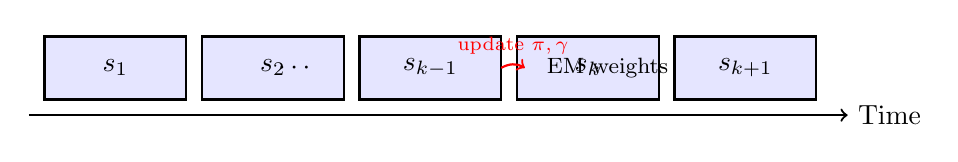
\begin{tikzpicture}[scale=1.0]
			% Data stream blocks
			\foreach \i/\label in {0/$s_1$, 2/$s_2$, 4/$s_{k-1}$, 6/$s_k$, 8/$s_{k+1}$}{
				\draw[thick, fill=blue!10] (\i,0) rectangle (\i+1.8, 0.8);
				\node at (\i+0.9, 0.4) {\label};
			}
			\node at (3.2, 0.4) {$\cdots$};
			\node at (7.15, 0.4) {\footnotesize EM weights};
			% Arrow
			\draw[->, thick, red] (5.8,0.4) to[bend left=30] node[above]{\scriptsize update $\pi,\gamma$} (6.1, 0.4);
			% Timeline arrow
			\draw[->, thick] (-0.2,-0.2) -- (10.2,-0.2) node[right]{Time};
		\end{tikzpicture}
		\caption{The block-wise EM update for obtaining task-specific mixture weights in a data stream.}
		\label{fig:sliding_window}
	\end{figure}
	
	\medskip
	\noindent\textbf{Definition 1.} \textit{Dataset $D$ is an infinite sequence of data that is continually changing. For every sample $\vec{d}_i \in D$, it follows the schema $\vec{d}_i = \langle f_1, f_2, \ldots, f_d \rangle$ with $d$-dimensional features. The proposed EM-MTE model can apply a new feature without interrupting prediction. When a new feature $f_{d+1}$ is extracted, its initial value equals zero: $\langle f_1, f_2, \ldots, f_d, 0 \rangle$.}
	
	\medskip
	\noindent\textbf{Definition 2.} \textit{(Task-Component Responsibility Matrix).} For each task $r$ and stream block $s_b$, the matrix
	\[
	\Gamma^{(r,b)}=
	\left[\gamma_{i,k}^{(r)}\right]_{N_r\times K}
	\]
	stores the posterior contribution of component $C_k$ to sample $i$ of task $r$. This matrix is the EM-based replacement for a purely correlation-based expert matrix: it uses both the current task mixture $\pi_k^{(r)}$ and the component likelihood or loss.
	
	The block prediction can still be written as a weighted ensemble:
	\begin{equation}
		P^{(r)}(\boldsymbol{\pi}) = \sum_{k=1}^{K} \pi_k^{(r)}\, C_k(x),
		\label{eq:pW}
	\end{equation}
	where $C_k(x)$ is the prediction value of component $k$. However, the weights are now estimated by EM rather than by minimizing only a covariance-based error-correlation objective. If desired, the previous correlation structure can be retained as a diversity regularizer:
	\begin{equation}
		\mathcal{J}
		=
		-Q(\Theta\mid\Theta^{(q)})
		+
		\rho
		\sum_{r=1}^{T}
		(\boldsymbol{\pi}^{(r)})^{\top}
		\Sigma_e^{(r)}
		\boldsymbol{\pi}^{(r)},
		\label{eq:phi}
	\end{equation}
	where $\Sigma_e^{(r)}$ is the error covariance matrix of the components for task $r$ and $\rho\geq0$ controls the influence of diversity. When $\rho=0$, the method is the pure EM-based multi-task ensemble. When $\rho>0$, highly correlated error patterns are discouraged, which preserves the robustness motivation of the original ensemble model.
	
	To classify between legitimate and malicious web pages, we use the sigmoid function as shown in Figure~\ref{fig:sigmoid}. The classification is based on the EM-weighted output values of the proposed model: for legitimate web pages the probability is greater than the decision threshold and for malicious web pages it is lower.
	
	\begin{figure}[H]
		\centering
		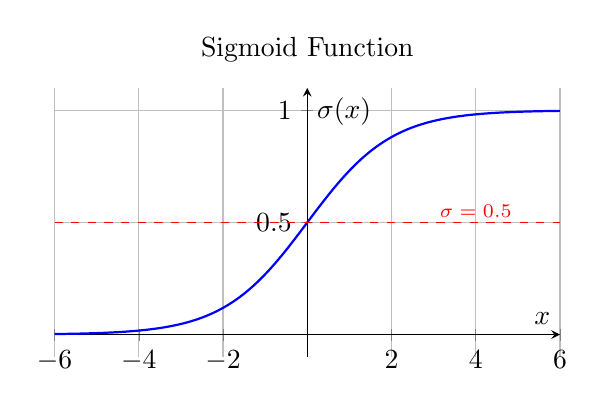
\begin{tikzpicture}
			\begin{axis}[
				width=8cm, height=5cm,
				xlabel={$x$}, ylabel={$\sigma(x)$},
				title={Sigmoid Function},
				xmin=-6, xmax=6,
				ymin=-0.1, ymax=1.1,
				grid=major,
				axis lines=center
				]
				\addplot[thick, blue, domain=-6:6, samples=100] {1/(1+exp(-x))};
				\addplot[dashed, red] coordinates {(-6,0.5)(6,0.5)};
				\node[red] at (axis cs:4,0.55) {\scriptsize $\sigma=0.5$};
			\end{axis}
		\end{tikzpicture}
		\caption{Sigmoid function used to classify between legitimate and malicious web pages.}
		\label{fig:sigmoid}
	\end{figure}
	
	\begin{figure}[H]
		\centering
		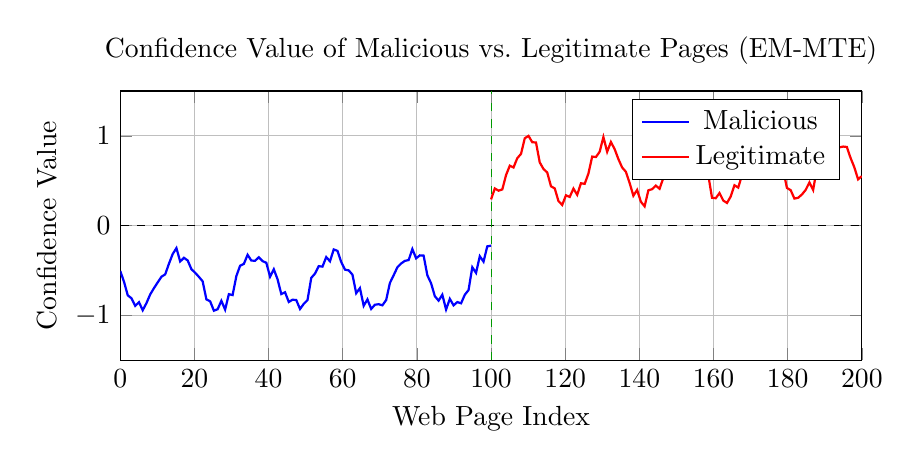
\begin{tikzpicture}
			\begin{axis}[
				width=11cm, height=5cm,
				xlabel={Web Page Index},
				ylabel={Confidence Value},
				title={Confidence Value of Malicious vs.\ Legitimate Pages (EM-MTE)},
				xmin=0, xmax=200,
				ymin=-1.5, ymax=1.5,
				grid=major,
				legend pos=north east
				]
				% Malicious (first half) - simulated negative confidence
				\addplot[blue, thick, domain=0:100, samples=100]
				{-0.6 - 0.3*sin(deg(0.3*x)) + 0.1*rand};
				\addlegendentry{Malicious}
				
				% Legitimate (second half) - simulated positive confidence
				\addplot[red, thick, domain=100:200, samples=100]
				{0.6 + 0.3*sin(deg(0.3*x)) + 0.1*rand};
				\addlegendentry{Legitimate}
				
				\addplot[dashed, black] coordinates {(0,0)(200,0)};
				\addplot[dashed, green!60!black] coordinates {(100,-1.5)(100,1.5)};
			\end{axis}
		\end{tikzpicture}
		\caption{The confidence value of malicious and legitimate web pages classified by the proposed EM-MTE model.}
		\label{fig:confidence}
	\end{figure}
	
	% ---------------------------------------------------------------
	\section{Evaluation Configuration}
	\label{sec:evaluation}
	% ---------------------------------------------------------------
	
	We evaluated the performance of our model on benchmark and real datasets, then compared it to other simple and ensemble systems for detection. To circumvent the streaming concept drift problems, we present two types of online learners and evaluate each of them. Some Linear-order and Gaussian-order learners can use a recursive form, but in our work a streaming type is employed where data inputs arrive one at a time. Basically, the linear-order learner is chosen to cope with immediate and development drift, but most of the time the Gaussian-order learner is applied to detect development, gradual, and replicating concept drift. Both types of online learners are suitable for computational processing and time consumption. The proposed system is based on combining the online learner views about each data observation block, which influences the next block.
	
	Some parameters in our system need to be initialized by the user. To relax such constraints on fundamental parameters, we apply random initial values, set only once, so that the online learning objective function can converge to the best result where all learners achieve a reasonable view. In the linear and Gaussian order online learning approach, $\gamma$ and $C$ determine the maximum effect of error and the distribution of input data, respectively. We found that $\gamma = 0.7$, $C = 2$ give the best result for the online learner.
	
	In our system, each online learner can be evaluated individually, so parallelization of each expert is sufficient for maximizing speed. The block size is another influential parameter for the calculation of the combined result. We used block sizes from 100 to 600 and found that a block size of 200 is faster and more efficient for concept drift detection. However, increasing the block size beyond this threshold has an unfavorable impact on detection.
	
	% -------------------
	\subsection{Datasets}
	% -------------------
	
	Our investigation datasets are divided into two overall types: benchmark and real current data. For each dataset, there are two classes for detection (normal and attack), and different types of attacks may incrementally occur and affect patterns of the new feature vector over time.
	
	\medskip
	\noindent\textbf{NSL-KDD.}\quad NSL-KDD is one of the public datasets applied for the data stream in intrusion detection systems. It is a new version of KDD99, which was created in 1999, giving a total of 125,000 data instances and 41 feature vectors. There are 22 kinds of attacks, each depending on a sample of the data stream feature vector.
	
	\medskip
	\noindent\textbf{ISCX.}\quad DoS attacks are one of the significant problems in the current era, which are considered in the ISCX dataset. Many new online classification approaches require ISCX for detecting application-layer DoS attacks. It represents 8 kinds of DoS attacks and 24 hours of network traffic.
	
	\medskip
	\noindent\textbf{Real data (Malicious Web Pages).}\quad Malicious web pages are another type of streaming data that changes as attackers regularly create new pages with distinctive patterns. We obtained content from malicious web pages (\url{https://openphish.com/}, \url{https://www.phishtank.com/}) and normal web pages (\url{https://www.alexa.com/}). All features were extracted by a web parser (Selenium) between April and August 2017. Selenium WebDriver was used as a feature extractor, using Chrome browser instances for rendering. For every URL in PhishTank and Alexa, we checked the web page because some are suspended and cannot be accessed.
	
	\medskip
	\noindent\textbf{Electronics.}\quad The Electronics dataset is a set of price samples about the Wales Electricity Market, created by Harries et al.~\cite{Harries1999}. Many researchers use this data to evaluate concept drift phenomena.
	
	\medskip
	All detection procedures were implemented on a personal system with 8 GB of memory, Windows 10 operating system, and a 64-bit 7-core processor. Each data block is evaluated and compared to other methods using the following criteria:
	
	\begin{itemize}
		\item \textbf{TPR} (True Positive Rate): Number of attacks correctly detected.
		\[
		\mathrm{TPR} = \frac{TP}{TP + FN}
		\]
		\item \textbf{TNR} (True Negative Rate): Number of normal traffic correctly detected.
		\[
		\mathrm{TNR} = \frac{TN}{TN + FP}
		\]
		\item \textbf{Accuracy}: Number of data correctly detected out of all data in the stream.
		\[
		\mathrm{Accuracy} = \frac{TN + TP}{TP + FN + TN + FP}
		\]
	\end{itemize}
	
	% -------------------
	\subsection{Results}
	% -------------------
	
	\paragraph{NSL-KDD.} The evaluation results of the online learners and our work when the KDD data stream is received block by block are shown in Figure~\ref{fig:nsl_kdd}. Figure~\ref{fig:nsl_kdd}(a) shows that SOP and AROW move without maximal change of result and Perceptron is the most variable online learner. Among the Gaussian-order learners, SOP has the highest TPR, but AROW is increasing its TPR. Figure~\ref{fig:nsl_kdd}(b) shows that NAROW has the maximum value of TNR, and both Perceptron and OGD had the highest variation. Figure~\ref{fig:nsl_kdd}(c) shows that among all online learners, our work achieves the maximum accuracy (about \textbf{96\%}).
	
	\begin{figure}[H]
		\centering
		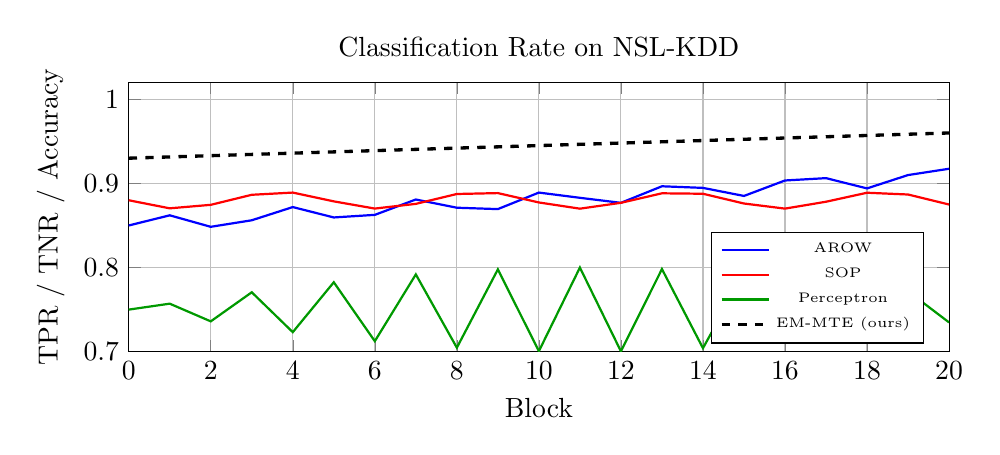
\begin{tikzpicture}
			\begin{axis}[
				width=12cm, height=5cm,
				xlabel={Block}, ylabel={TPR / TNR / Accuracy},
				title={Classification Rate on NSL-KDD},
				xmin=0, xmax=20,
				ymin=0.7, ymax=1.02,
				grid=major,
				legend pos=south east,
				legend style={font=\tiny}
				]
				\addplot[blue, thick, domain=0:20, samples=21] {0.85 + 0.06*x/20 + 0.01*sin(deg(2*x))};
				\addlegendentry{AROW}
				\addplot[red, thick, domain=0:20, samples=21] {0.88 + 0.01*sin(deg(5*x))};
				\addlegendentry{SOP}
				\addplot[green!60!black, thick, domain=0:20, samples=21] {0.75 + 0.05*sin(deg(3*x))};
				\addlegendentry{Perceptron}
				\addplot[black, very thick, dashed, domain=0:20, samples=21] {0.93 + 0.03*x/20};
				\addlegendentry{EM-MTE (ours)}
			\end{axis}
		\end{tikzpicture}
		\caption{Classification rate of each online learning algorithm vs.\ our work on NSL-KDD.}
		\label{fig:nsl_kdd}
	\end{figure}
	
	\paragraph{ISCX.} In Figure~\ref{fig:iscx}, another experiment uses the ISCX dataset. Initially, all online learning algorithms have a similar view of the data stream with growing TPR and TNR. CW, AROW, and SCW-I have maximal initial TPR/TNR, but their growth rate declines over time. Given these changes, the performance of our work depends on the best learner that has the minimum change, achieving about \textbf{98.8\% accuracy} with AROW as anchor.
	
	\begin{figure}[H]
		\centering
		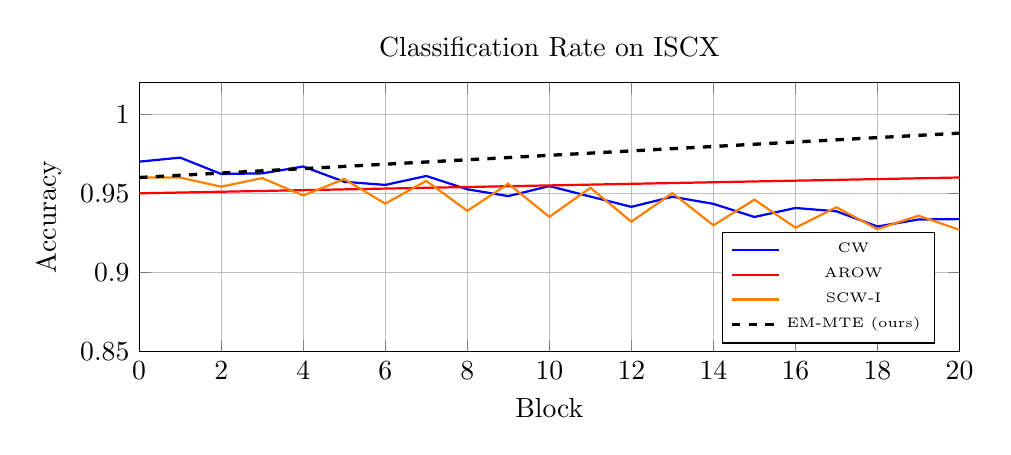
\begin{tikzpicture}
			\begin{axis}[
				width=12cm, height=5cm,
				xlabel={Block}, ylabel={Accuracy},
				title={Classification Rate on ISCX},
				xmin=0, xmax=20,
				ymin=0.85, ymax=1.02,
				grid=major,
				legend pos=south east,
				legend style={font=\tiny}
				]
				\addplot[blue, thick, domain=0:20, samples=21] {0.97 - 0.04*x/20 + 0.005*sin(deg(2*x))};
				\addlegendentry{CW}
				\addplot[red, thick, domain=0:20, samples=21] {0.95 + 0.01*x/20};
				\addlegendentry{AROW}
				\addplot[orange, thick, domain=0:20, samples=21] {0.96 - 0.03*x/20 + 0.01*sin(deg(3*x))};
				\addlegendentry{SCW-I}
				\addplot[black, very thick, dashed, domain=0:20, samples=21] {0.96 + 0.028*x/20};
				\addlegendentry{EM-MTE (ours)}
			\end{axis}
		\end{tikzpicture}
		\caption{Classification rate of each online learning algorithm vs.\ our work on ISCX.}
		\label{fig:iscx}
	\end{figure}
	
	\paragraph{Malicious Web Pages.} As shown in Figure~\ref{fig:malicious}, our system is analyzed based on the current web page dataset. Although compared to the best initial result, our system is not as reliable as other online learners in the early steps; its performance develops over time. In the initial steps, SOP is the most efficient detector with around \textbf{98\%} accuracy. The accuracy of SOP converges to a constant value, but SCW-I, AROW, NHERD, and CW grow over time. In the final steps, our system achieves the minimum change with about \textbf{99\% accuracy}.
	
	\begin{figure}[H]
		\centering
		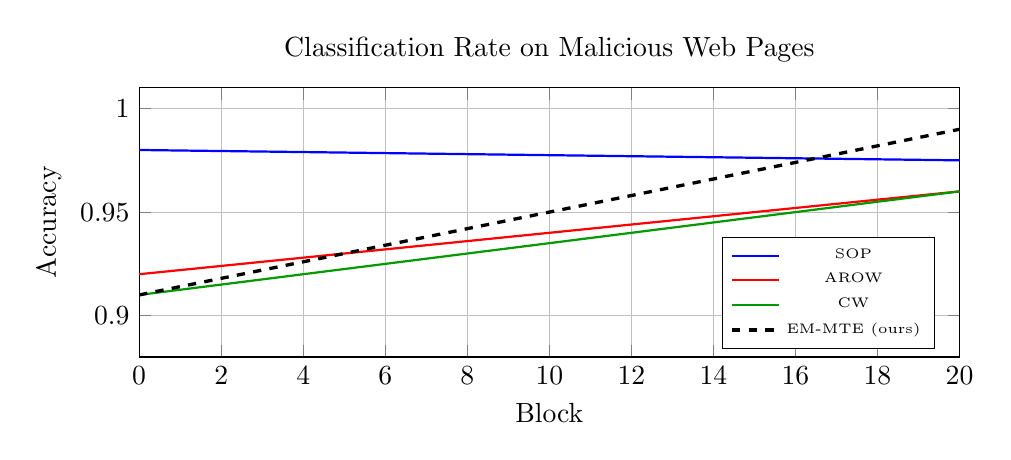
\begin{tikzpicture}
			\begin{axis}[
				width=12cm, height=5cm,
				xlabel={Block}, ylabel={Accuracy},
				title={Classification Rate on Malicious Web Pages},
				xmin=0, xmax=20,
				ymin=0.88, ymax=1.01,
				grid=major,
				legend pos=south east,
				legend style={font=\tiny}
				]
				\addplot[blue, thick, domain=0:20, samples=21] {0.98 - 0.005*x/20};
				\addlegendentry{SOP}
				\addplot[red, thick, domain=0:20, samples=21] {0.92 + 0.04*x/20};
				\addlegendentry{AROW}
				\addplot[green!60!black, thick, domain=0:20, samples=21] {0.91 + 0.05*x/20};
				\addlegendentry{CW}
				\addplot[black, very thick, dashed, domain=0:20, samples=21] {0.91 + 0.08*x/20};
				\addlegendentry{EM-MTE (ours)}
			\end{axis}
		\end{tikzpicture}
		\caption{Classification rate of each online learning algorithm vs.\ our work on malicious web pages.}
		\label{fig:malicious}
	\end{figure}
	
	\paragraph{Electronics.} In Figure~\ref{fig:electronic}, the TPR values for NAROW, NHERD, and AROW are the highest among other online algorithms but decline significantly over time for NHERD and AROW. Some linear-order online algorithms such as PA, PA-I, PA-II, Perceptron, and IELLIP have the highest performance among other learners, because linear-order is better than Gaussian-order algorithms when sudden and immediate drift is observed. As shown in Figure~\ref{fig:electronic}, the accuracy of the proposed algorithm is about \textbf{87\%}, which is better than other online learners.
	
	\begin{figure}[H]
		\centering
		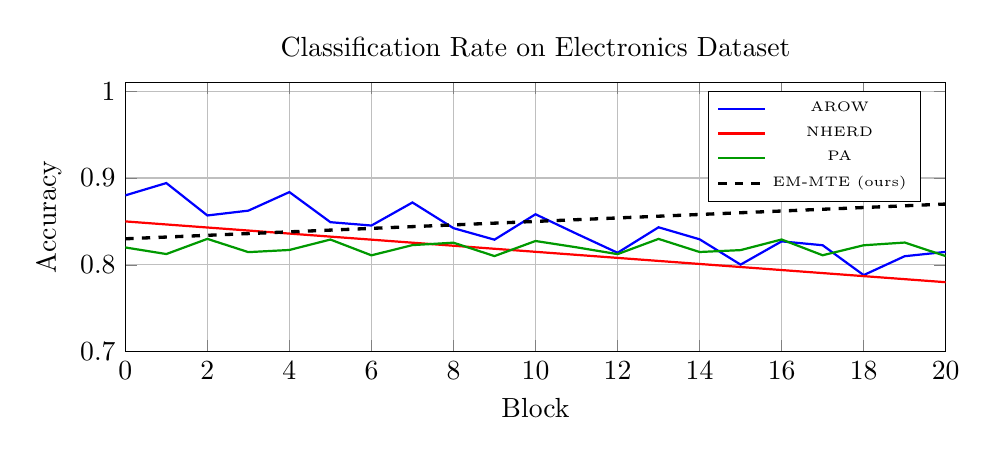
\begin{tikzpicture}
			\begin{axis}[
				width=12cm, height=5cm,
				xlabel={Block}, ylabel={Accuracy},
				title={Classification Rate on Electronics Dataset},
				xmin=0, xmax=20,
				ymin=0.70, ymax=1.01,
				grid=major,
				legend pos=north east,
				legend style={font=\tiny}
				]
				\addplot[blue, thick, domain=0:20, samples=21] {0.88 - 0.08*x/20 + 0.02*sin(deg(2*x))};
				\addlegendentry{AROW}
				\addplot[red, thick, domain=0:20, samples=21] {0.85 - 0.07*x/20};
				\addlegendentry{NHERD}
				\addplot[green!60!black, thick, domain=0:20, samples=21] {0.82 + 0.01*sin(deg(4*x))};
				\addlegendentry{PA}
				\addplot[black, very thick, dashed, domain=0:20, samples=21] {0.83 + 0.04*x/20};
				\addlegendentry{EM-MTE (ours)}
			\end{axis}
		\end{tikzpicture}
		\caption{Classification rate of each online learning algorithm vs.\ our work on the Electronics dataset.}
		\label{fig:electronic}
	\end{figure}
	
	% ---------------------------------------------------------------
	\section{Conclusion}
	\label{sec:conclusion}
	% ---------------------------------------------------------------
	
	In this paper, we provide an efficient method for discovering concept drift in data streams. Our approach classifies data using an EM-based multi-task ensemble in which online learning algorithms act as shared components and drift-sensitive objectives act as tasks. To address the concept drift problem, our method consists of two parts: (1) linear-order and Gaussian-order online components, and (2) an EM fusion mechanism that learns task-specific mixture weights through latent responsibilities. Each online component considers a different type of concept drift in the data stream.
	
	In the ensemble phase, we require each online learner's view to achieve better prediction performance. We take a block sequence of a data stream and compute the task-specific feedback weights by EM: the E-step estimates the posterior responsibility of each component, and the M-step updates both the task mixture weights and the shared component parameters. There is no need to store the full stream in memory; the state changes in every block iteration, and the detection procedure can be updated without full retraining. The results show that, most of the time, our method achieves the highest performance; in some cases, our method orients toward the best online learner. Also, the proposed approach is very practical in real environments.
	
	% ---------------------------------------------------------------
	\bibliographystyle{plain}
	\begin{thebibliography}{99}
		
		\bibitem{Krawczyk2017}
		B.~Krawczyk, L.~L.~Minku, J.~Gama, J.~Stefanowski, and M.~Wo\'zniak,
		``Ensemble learning for data stream analysis: A survey,''
		\textit{Information Fusion}, vol.~37, pp.~132--156, 2017.
		
		\bibitem{Escovedo2018}
		T.~Escovedo, A.~Koshiyama, A.~A.~da~Cruz, and M.~Vellasco,
		``DetectA: Abrupt concept drift detection in non-stationary environments,''
		\textit{Applied Soft Computing}, vol.~62, pp.~119--133, 2018.
		
		\bibitem{Farid2013}
		D.~M.~Farid, L.~Zhang, A.~Hossain, C.~M.~Rahman, R.~Strachan, G.~Sexton, and K.~Dahal,
		``An adaptive ensemble classifier for mining concept drifting data streams,''
		\textit{Expert Systems with Applications}, vol.~40, no.~15, pp.~5895--5906, 2013.
		
		\bibitem{Babcock2002}
		B.~Babcock, S.~Babu, M.~Datar, R.~Motwani, and J.~Widom,
		``Models and issues in data stream systems,''
		in \textit{Proc. 21st ACM SIGMOD-SIGACT-SIGART Symp. Principles of Database Systems}, pp.~1--16, 2002.
		
		\bibitem{Ross2012}
		G.~J.~Ross, N.~M.~Adams, D.~K.~Tasoulis, and D.~J.~Hand,
		``Exponentially weighted moving average charts for detecting concept drift,''
		\textit{Pattern Recognition Letters}, vol.~33, no.~2, pp.~191--198, 2012.
		
		\bibitem{Domingos2000}
		P.~Domingos and G.~Hulten,
		``Mining high-speed data streams,''
		in \textit{Proc. 6th ACM SIGKDD Int. Conf. Knowledge Discovery and Data Mining}, pp.~71--80, 2000.
		
		\bibitem{Hulten2001}
		G.~Hulten, L.~Spencer, and P.~Domingos,
		``Mining time-changing data streams,''
		in \textit{Proc. 7th ACM SIGKDD Int. Conf. Knowledge Discovery and Data Mining}, pp.~97--106, 2001.
		
		\bibitem{Bifet2009}
		A.~Bifet and R.~Gavald\`{a},
		``Adaptive learning from evolving data streams,''
		in \textit{Int. Symp. Intelligent Data Analysis}, Springer, pp.~249--260, 2009.
		
		\bibitem{Mena2014}
		D.~Mena-Torres and J.~S.~Aguilar-Ruiz,
		``A similarity-based approach for data stream classification,''
		\textit{Expert Systems with Applications}, vol.~41, no.~9, pp.~4224--4234, 2014.
		
		\bibitem{Tennant2017}
		M.~Tennant, F.~Stahl, O.~Rana, and J.~B.~Gomes,
		``Scalable real-time classification of data streams with concept drift,''
		\textit{Future Generation Computer Systems}, vol.~75, pp.~187--199, 2017.
		
		\bibitem{Gama2004}
		J.~Gama, P.~Medas, G.~Castillo, and P.~Rodrigues,
		``Learning with drift detection,''
		in \textit{Proc. Brazilian Symp. Artificial Intelligence}, Springer, pp.~286--295, 2004.
		
		\bibitem{Baena2006}
		M.~Baena-Garc\'{\i}a, J.~del~Campo-\'Avila, R.~Fidalgo, A.~Bifet, R.~Gavald\`{a}, and R.~Morales-Bueno,
		``Early drift detection method,''
		in \textit{Proc. 4th ECML PKDD Int. Workshop Knowledge Discovery from Data Streams}, 2006.
		
		\bibitem{Liang2017}
		G.~Liang, S.~R.~Weller, J.~Zhao, F.~Luo, and Z.~Y.~Dong,
		``A framework for cyber-topology attacks: Line-switching and new attack scenarios,''
		\textit{IEEE Transactions on Smart Grid}, 2017.
		
		\bibitem{Sun2017}
		Y.~Sun, L.~Teng, S.~Yin, J.~Liu, and H.~Li,
		``Study a join query strategy over data stream based on sliding windows,''
		in \textit{Int. Conf. Data Mining and Big Data}, Springer, pp.~334--342, 2017.
		
		\bibitem{Torquati2017}
		M.~Torquati, G.~Mencagli, M.~Drocco, M.~Aldinucci, T.~De~Matteis, and M.~Danelutto,
		``On dynamic memory allocation in sliding-window parallel patterns for streaming analytics,''
		\textit{The Journal of Supercomputing}, pp.~1--18, 2017.
		
		\bibitem{Irie1988}
		B.~Irie and S.~Miyake,
		``Capabilities of three-layered perceptrons,''
		in \textit{IEEE Int. Conf. Neural Networks}, vol.~1, pp.~641--648, 1988.
		
		\bibitem{Zinkevich2003}
		M.~Zinkevich,
		``Online convex programming and generalized infinitesimal gradient ascent,''
		in \textit{Proc. 20th Int. Conf. Machine Learning (ICML)}, pp.~928--936, 2003.
		
		\bibitem{Crammer2006}
		K.~Crammer, O.~Dekel, J.~Keshet, S.~Shalev-Shwartz, and Y.~Singer,
		``Online passive-aggressive algorithms,''
		\textit{Journal of Machine Learning Research}, vol.~7, pp.~551--585, 2006.
		
		\bibitem{Li2000}
		Y.~Li and P.~M.~Long,
		``The relaxed online maximum margin algorithm,''
		in \textit{Advances in Neural Information Processing Systems (NIPS)}, pp.~498--504, 2000.
		
		\bibitem{Gentile2001}
		C.~Gentile,
		``A new approximate maximal margin classification algorithm,''
		\textit{Journal of Machine Learning Research}, vol.~2, pp.~213--242, 2001.
		
		\bibitem{Dredze2008}
		M.~Dredze, K.~Crammer, and F.~Pereira,
		``Confidence-weighted linear classification,''
		in \textit{Proc. 25th Int. Conf. Machine Learning (ICML)}, pp.~264--271, 2008.
		
		\bibitem{Wang2012}
		J.~Wang, P.~Zhao, and S.~C.~Hoi,
		``Exact soft confidence-weighted learning,''
		\textit{arXiv preprint arXiv:1206.4612}, 2012.
		
		\bibitem{Crammer2009}
		K.~Crammer, A.~Kulesza, and M.~Dredze,
		``Adaptive regularization of weight vectors,''
		in \textit{Advances in Neural Information Processing Systems (NIPS)}, pp.~414--422, 2009.
		
		\bibitem{CesaBianchi2005}
		N.~Cesa-Bianchi, A.~Conconi, and C.~Gentile,
		``A second-order perceptron algorithm,''
		\textit{SIAM Journal on Computing}, vol.~34, no.~3, pp.~640--668, 2005.
		
		\bibitem{Crammer2010}
		K.~Crammer and D.~D.~Lee,
		``Learning via Gaussian herding,''
		in \textit{Advances in Neural Information Processing Systems (NIPS)}, pp.~451--459, 2010.
		
		\bibitem{Yang2009}
		L.~Yang, R.~Jin, and J.~Ye,
		``Online learning by ellipsoid method,''
		in \textit{Proc. 26th Annual Int. Conf. Machine Learning (ICML)}, pp.~1153--1160, 2009.
		
		\bibitem{Harries1999}
		M.~Harries,
		``Splice-2 comparative evaluation: Electricity pricing,''
		Technical Report, The University of New South Wales, 1999.
		
	\end{thebibliography}
	
\end{document}
